\documentclass{report}
\usepackage[utf8]{inputenc}


\usepackage[a4paper, total={6in, 8in}]{geometry}


\title{Entwiklung Algorithmus Obere Halswirbelsäule}
\author{Lukas Hörnig}
\date{Oktober 2017}

\usepackage[square,sort,comma,numbers]{natbib}
\usepackage{graphicx}
\usepackage{hyperref}
\usepackage{gensymb}

\begin{document}

\section{Basion Dens Inteval}
\subsection{Definiton}
\begin{figure}
        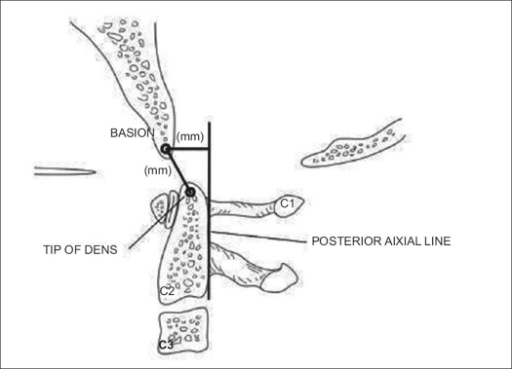
\includegraphics[width=8cm]{BDI.png}
\end{figure}
Definiert als Länge der kürzesten Distanz zwischen dem Mittelpunkt des Basion und der Spitze des Dens in sagitaler Mittelininerekonstruktion in Millimetern.


\subsection{Statistik}
Das BDI zeigt über die Altersgruppen und Geschlechter keine nennenswerte Instabilität \cite{Chaput2011} und wurde schon bezüglich Normwerte und pathologischer Abweichung ausgiebig untersucht.
\cite{Radcliff2010,Radcliff2012,Chang2009,Harris1994,Harris1994a,Chaput2011,Rojas2007,Gonzalez2004,Gonzalez2004a,Dziurzynski2005,Bono2007}. 



\paragraph{Validität}
% Resultiert aus Dislokation Instabilität??
Sowohl für die Sensibilität als auch für die Spezifität bezüglich des BDI für Atlanto-occipitale Dislokation und daraus resultierender Instabilität zeigen sich eine hohe Güte \cite{Dziurzynski2005}.

\paragraph{Reliabiliät}
% Hier fehlen noch die genauen Berechnungsformen und Kappa werte PDF-Chapter 6
Der BDI zeigt sich sowohl bezüglich Intra- und Interobserver Reliabiliät eine sehr hohe Güte \cite{Chaput2011,Dziurzynski2005,Harris1994,Harris1994a}, welche durch stabile Verhältnisse und verbesserte Bildgebung, sowie deren Lesbarkeit, welche durch verlässliche Darstellung der benötigten anatomischen Landmarken garantiert werden \cite{Dziurzynski2005,Radcliff2010}.


\subsection{Patholgischer Wert}
Ab einem Wert von 


\subsection{Anwendbarkeit}
Die Anwendbarkeit wird bei Messung an CT-Bildgebung durch hochaufgelöste, überlagerungsfreie Darstellung für erfahrene Anwender der Technik sehr zuverlässig und in fast allen Fällen möglich gemacht \cite{Dziurzynski2005,Radcliff2010}. 


\section{LMI}
Das LMI zeigt über Altersgruppen und Geschlechter hinweg eine statistisch signifiktante Instabilität \cite{Chaput2011}

\bibliography{../literatur}
\bibliographystyle{dinat}
\end{document}
